\documentclass[11pt,a4paper]{report}
\usepackage[textwidth=37em,vmargin=30mm]{geometry}
\usepackage{calc,xunicode,amsmath,amssymb,paralist,enumitem,tabu,booktabs,datetime2,xeCJK,xeCJKfntef,listings}
\usepackage{tocloft,fancyhdr,tcolorbox,xcolor,graphicx,eso-pic,xltxtra,xelatexemoji}

\newcommand{\envyear}[0]{2025}
\newcommand{\envdatestr}[0]{2025-11-02}
\newcommand{\envfinaldir}[0]{webdb/2025/20251102/final}

\usepackage[hidelinks]{hyperref}
\hypersetup{
    colorlinks=false,
    pdfpagemode=FullScreen,
    pdftitle={Web Digest - \envdatestr}
}

\setlength{\cftbeforechapskip}{10pt}
\renewcommand{\cftchapfont}{\rmfamily\bfseries\large\raggedright}
\setlength{\cftbeforesecskip}{2pt}
\renewcommand{\cftsecfont}{\sffamily\small\raggedright}

\setdefaultleftmargin{2em}{2em}{1em}{1em}{1em}{1em}

\usepackage{xeCJK,xeCJKfntef}
\xeCJKsetup{PunctStyle=plain,RubberPunctSkip=false,CJKglue=\strut\hskip 0pt plus 0.1em minus 0.05em,CJKecglue=\strut\hskip 0.22em plus 0.2em}
\XeTeXlinebreaklocale "zh"
\XeTeXlinebreakskip = 0pt


\setmainfont{Brygada 1918}
\setromanfont{Brygada 1918}
\setsansfont{IBM Plex Sans}
\setmonofont{JetBrains Mono NL}
\setCJKmainfont{Noto Serif CJK SC}
\setCJKromanfont{Noto Serif CJK SC}
\setCJKsansfont{Noto Sans CJK SC}
\setCJKmonofont{Noto Sans CJK SC}

\setlength{\parindent}{0pt}
\setlength{\parskip}{8pt}
\linespread{1.15}

\lstset{
	basicstyle=\ttfamily\footnotesize,
	numbersep=5pt,
	backgroundcolor=\color{black!5},
	showspaces=false,
	showstringspaces=false,
	showtabs=false,
	tabsize=2,
	captionpos=b,
	breaklines=true,
	breakatwhitespace=true,
	breakautoindent=true,
	linewidth=\textwidth
}






\newcommand{\coverpic}[2]{
    % argv: itemurl, authorname
    Cover photo by #2~~(\href{#1}{#1})
}
\newcommand{\makeheader}[0]{
    \begin{titlepage}
        % \newgeometry{hmargin=15mm,tmargin=21mm,bmargin=12mm}
        \begin{center}
            
            \rmfamily\scshape
            \fontspec{BaskervilleF}
            \fontspec{Old Standard}
            \fontsize{59pt}{70pt}\selectfont
            WEB\hfill DIGEST
            
            \vfill
            % \vskip 30pt
            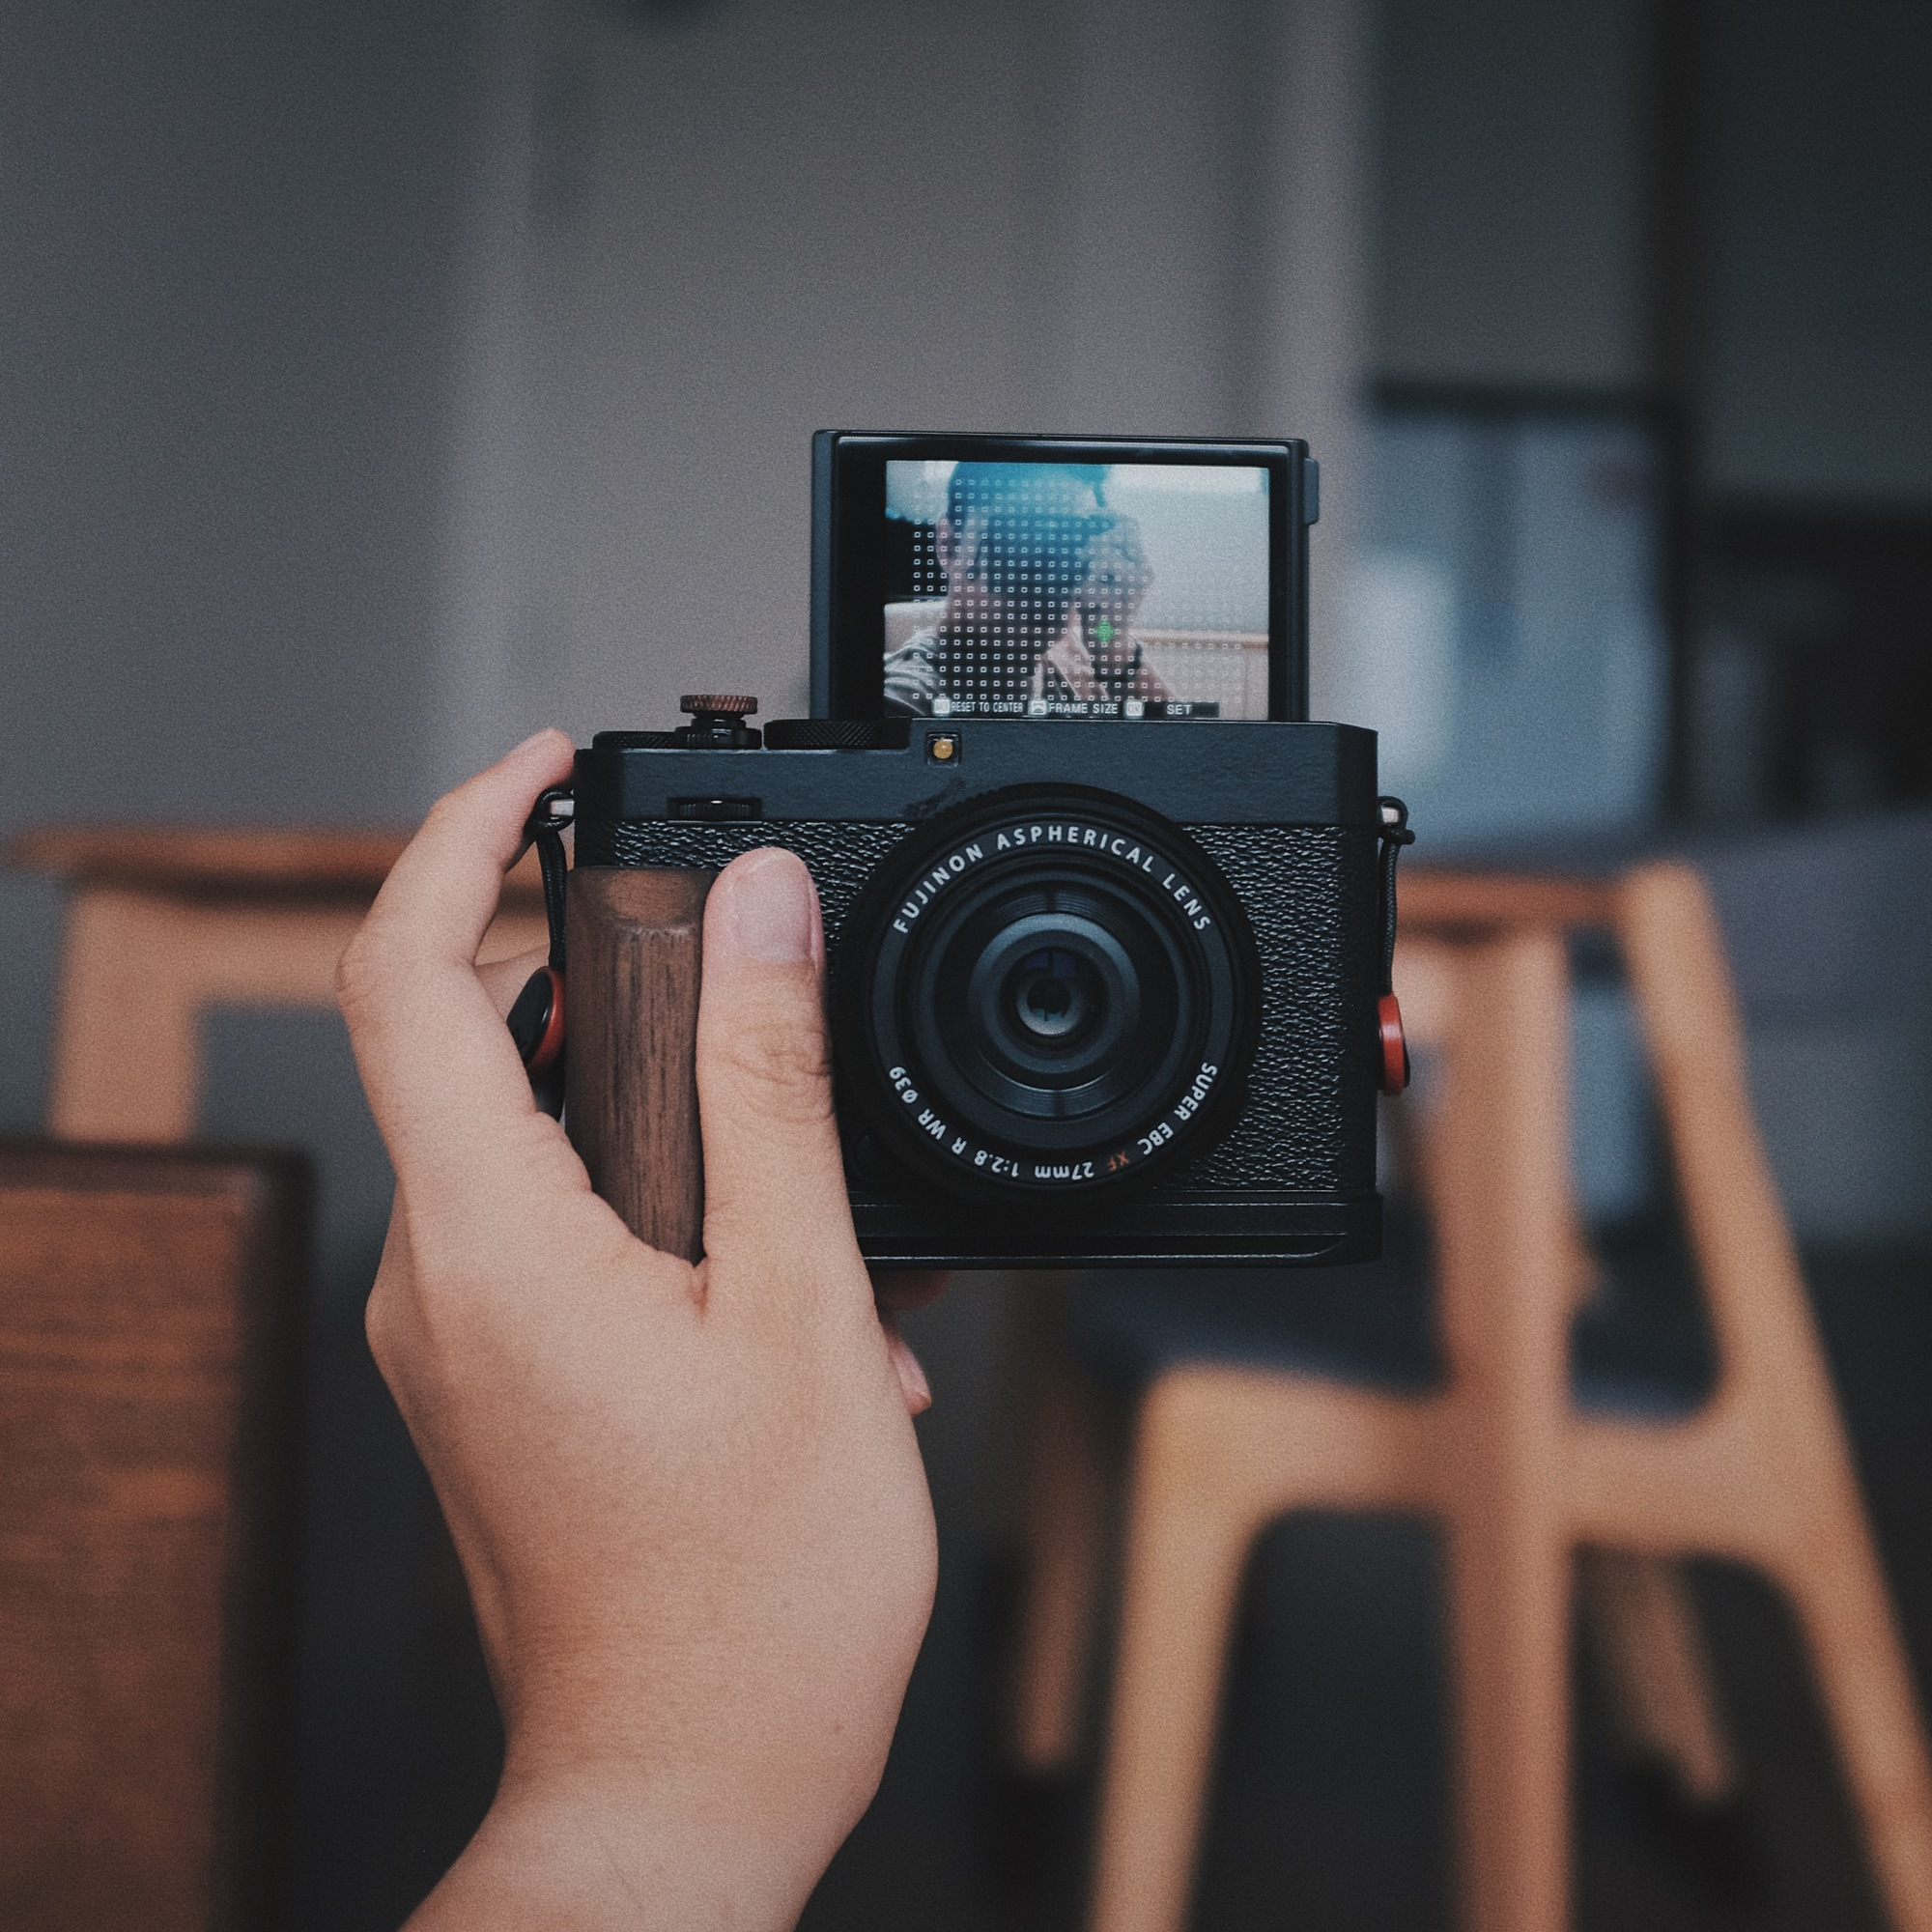
\includegraphics[width=\linewidth]{\envfinaldir/coverpic-prod.jpg}\par
            % \vskip 30pt
            \vfill

            \normalsize\rmfamily\scshape
            \copyright{} The Web Digest Project \hfill\large \envdatestr
        \end{center}
    \end{titlepage}
    % \restoregeometry
}
\newcommand{\simplehref}[1]{%
    \textcolor{blue!80!green}{\href{#1}{#1}}%
}
\renewcommand{\contentsname}{\center\Huge\sffamily\bfseries Contents\par\vskip 20pt}
\newcounter{ipartcounter}
\setcounter{ipartcounter}{0}
\newcommand{\ipart}[1]{
    % \vskip 20pt
    \clearpage
    \stepcounter{ipartcounter}
    \phantomsection
    \addcontentsline{toc}{chapter}{#1}
    % \begin{center}
    %     \Huge
    %     \sffamily\bfseries
    %     #1
    % \end{center}
    % \vskip 20pt plus 7pt
}
\newcounter{ichaptercounter}
\setcounter{ichaptercounter}{0}
\newcommand{\ichapter}[1]{
    % \vskip 20pt
    \clearpage
    \stepcounter{ichaptercounter}
    \phantomsection
    \addcontentsline{toc}{section}{\numberline{\arabic{ichaptercounter}}#1}
    \begin{center}
        \Huge
        \sffamily\bfseries
        #1
    \end{center}
    \vskip 20pt plus 7pt
}
\newcommand{\entrytitlefont}[1]{\subsection*{\raggedright\Large\sffamily\bfseries#1}}
\newcommand{\entryitemGeneric}[2]{
    % argv: title, url
    \parbox{\linewidth}{
        \entrytitlefont{#1}\par\vskip 5pt
        \footnotesize\ttfamily\mdseries
        \simplehref{#2}
    }\vskip 11pt plus 11pt minus 1pt
}
\newcommand{\entryitemGithub}[3]{
    % argv: title, url, desc
    \parbox{\linewidth}{
        \entrytitlefont{#1}\par\vskip 5pt
        \footnotesize\ttfamily\mdseries
        \simplehref{#2}\par\vskip 5pt
        \small\rmfamily\mdseries#3
    }\vskip 11pt plus 11pt minus 1pt
}
\newcommand{\entryitemAp}[3]{
    % argv: title, url, desc
    \parbox{\linewidth}{
        \entrytitlefont{#1}\par\vskip 5pt
        \footnotesize\ttfamily\mdseries
        \simplehref{#2}\par\vskip 5pt
        \small\rmfamily\mdseries#3
    }\vskip 11pt plus 11pt minus 1pt
}
\newcommand{\entryitemHackernews}[3]{
    % argv: title, hnurl, rawurl
    % \parbox{\linewidth}{
    %     \entrytitlefont{#1}\par\vskip 5pt
    %     \footnotesize\ttfamily\mdseries
    %     \simplehref{#3}\par
    %     \textcolor{black!50}{\href{#2}{#2}}
    % }\vskip 11pt plus 11pt minus 1pt
    \begin{minipage}{\linewidth}
            \entrytitlefont{#1}\par\vskip 5pt
            \footnotesize\ttfamily\mdseries
            \simplehref{#3}\par
            \textcolor{black!50}{\href{#2}{#2}}
    \end{minipage}\par\vskip 11pt plus 11pt minus 1pt
}







\begin{document}

\makeheader

\tableofcontents\clearpage




\ipart{Developers}
\ichapter{Hacker News}
\entryitemTwoLinks{SailfishOS: A Linux-based European alternative to dominant mobile OSes}{https://news.ycombinator.com/item?id=45785840}{https://sailfishos.org/info/}

\entryitemTwoLinks{Claude Code Can Debug Low-Level Cryptography}{https://news.ycombinator.com/item?id=45784179}{https://words.filippo.io/claude-debugging/}

\entryitemTwoLinks{Visible from space, Sudan's bloodied sands expose a massacre of thousands}{https://news.ycombinator.com/item?id=45783699}{https://www.telegraph.co.uk/world-news/2025/10/28/sudan-bloodied-sands-massacre-thousands/}

\entryitemTwoLinks{Show HN: Why write code if the LLM can just do the thing? (web app experiment)}{https://news.ycombinator.com/item?id=45783640}{https://github.com/samrolken/nokode}

\entryitemTwoLinks{OpenAI Moves to Complete Potentially the Largest Theft in Human History}{https://news.ycombinator.com/item?id=45783470}{https://thezvi.substack.com/p/openai-moves-to-complete-potentially}

\entryitemTwoLinks{Studies increasingly find links between air pollutants and dementia}{https://news.ycombinator.com/item?id=45783206}{https://www.nytimes.com/2025/11/01/health/alzheimers-dementia-air-pollution.html}

\entryitemTwoLinks{Chat Control proposal fails again after public opposition}{https://news.ycombinator.com/item?id=45783114}{https://andreafortuna.org/2025/11/01/chat-control-proposal-fails-again-after-massive-public-opposition/}

\entryitemTwoLinks{GHC now runs in the browser}{https://news.ycombinator.com/item?id=45782981}{https://discourse.haskell.org/t/ghc-now-runs-in-your-browser/13169}

\entryitemTwoLinks{Tech companies are firing everyone to "fund AI", spending money on each other}{https://news.ycombinator.com/item?id=45782267}{https://old.reddit.com/r/ArtificialInteligence/comments/1oj52xx/tech\_companies\_are\_firing\_everyone\_to\_fund\_ai\_but/}

\entryitemTwoLinks{Updated practice for review articles and position papers in ArXiv CS category}{https://news.ycombinator.com/item?id=45782136}{https://blog.arxiv.org/2025/10/31/attention-authors-updated-practice-for-review-articles-and-position-papers-in-arxiv-cs-category/}

\entryitemTwoLinks{CharlotteOS – An Experimental Modern Operating System}{https://news.ycombinator.com/item?id=45781397}{https://github.com/charlotte-os/Catten}

\entryitemTwoLinks{SQLite concurrency and why you should care about it}{https://news.ycombinator.com/item?id=45781298}{https://jellyfin.org/posts/SQLite-locking/}

\entryitemTwoLinks{Do you know that there is an HTML tables API?}{https://news.ycombinator.com/item?id=45781293}{https://christianheilmann.com/2025/10/08/abandonware-of-the-web-do-you-know-that-there-is-an-html-tables-api/}

\entryitemTwoLinks{You can't refuse to be scanned by ICE's facial recognition app, DHS document say}{https://news.ycombinator.com/item?id=45780228}{https://www.404media.co/you-cant-refuse-to-be-scanned-by-ices-facial-recognition-app-dhs-document-says/}

\entryitemTwoLinks{Hard Rust requirements from May onward}{https://news.ycombinator.com/item?id=45779860}{https://lists.debian.org/debian-devel/2025/10/msg00285.html}

\entryitemTwoLinks{The profitable startup}{https://news.ycombinator.com/item?id=45778984}{https://linear.app/now/the-profitable-startup}

\entryitemTwoLinks{Show HN: Strange Attractors}{https://news.ycombinator.com/item?id=45777810}{https://blog.shashanktomar.com/posts/strange-attractors}

\entryitemTwoLinks{S.A.R.C.A.S.M: Slightly Annoying Rubik's Cube Automatic Solving Machine}{https://news.ycombinator.com/item?id=45777682}{https://github.com/vindar/SARCASM}

\entryitemTwoLinks{Tim Bray on Grokipedia}{https://news.ycombinator.com/item?id=45777015}{https://www.tbray.org/ongoing/When/202x/2025/10/28/Grokipedia}

\entryitemTwoLinks{A theoretical way to circumvent Android developer verification}{https://news.ycombinator.com/item?id=45776269}{https://enaix.github.io/2025/10/30/developer-verification.html}\ichapter{Phoronix}
\entryitemGeneric{\hskip 0pt{}Debian's APT Will Soon Begin Requiring Rust: Debian Ports Need To Adapt Or Be Sunset}{https://www.phoronix.com/news/Debian-APT-Will-Require-Rust}

\entryitemGeneric{\hskip 0pt{}Linux Kernel Ported To WebAssembly - Demo Lets You Run It In Your Web Browser}{https://www.phoronix.com/news/Linux-Kernel-WebAssembly}

\entryitemGeneric{\hskip 0pt{}Archinstall 3.0.12 \& Pacman 7.1 Released For Arch Linux Users}{https://www.phoronix.com/news/Archinstall-3.0.12-Pacman-7.1}

\entryitemGeneric{\hskip 0pt{}PCI Resizable BAR Improvements Heading To Linux 6.19}{https://www.phoronix.com/news/PCI-ReBAR-Better-Linux-6.19}

\entryitemGeneric{\hskip 0pt{}Linux 6.18 Kernel Happenings, Python 3.14, NTFSPLUS \& Other October Highlights}{https://www.phoronix.com/news/October-2025-Highlights}

\entryitemGeneric{\hskip 0pt{}AMD Acknowledges RDSEED Failure On AMD Zen 5 With Software Fix Coming}{https://www.phoronix.com/news/AMD-SB-7055-RDSEED-Zen-5}

\entryitemGeneric{\hskip 0pt{}KDE Plasma 6.6 To Support Intel's Adaptive Sharpness Feature}{https://www.phoronix.com/news/Plasma-6.6-Adaptive-Sharpness}

\entryitemGeneric{\hskip 0pt{}Wine 10.18 Released With More WoW64 Mode Improvements}{https://www.phoronix.com/news/Wine-10.18-Released}

\entryitemGeneric{\hskip 0pt{}GNOME Gains A New macOS-Inspired Quick Menu Option}{https://www.phoronix.com/news/GNOME-Kiwi-macOS-Quick-Menu}


\ipart{Developers~~~~(zh-Hans)}
\ichapter{Solidot}
\entryitemGeneric{\hskip 0pt{}特朗普命令美国重启核武器试验}{https://www.solidot.org/story?sid=82688}

\entryitemGeneric{\hskip 0pt{}Bazzite 秋季更新释出}{https://www.solidot.org/story?sid=82687}

\entryitemGeneric{\hskip 0pt{}以色列要求 Google 和亚马逊使用秘密的眨眼信号警告外国政府的数据披露要求}{https://www.solidot.org/story?sid=82686}

\entryitemGeneric{\hskip 0pt{}英国面临禁止汞合金填充物的压力}{https://www.solidot.org/story?sid=82685}

\entryitemGeneric{\hskip 0pt{}Affinity Studio 成为免费软件 }{https://www.solidot.org/story?sid=82684}

\entryitemGeneric{\hskip 0pt{}数学证明否定宇宙是模拟的}{https://www.solidot.org/story?sid=82683}

\entryitemGeneric{\hskip 0pt{}DNS 运行在 FOSS 之上}{https://www.solidot.org/story?sid=82682}

\entryitemGeneric{\hskip 0pt{}社会最终会接受自动驾驶出租车导致的致命车祸}{https://www.solidot.org/story?sid=82681}

\entryitemGeneric{\hskip 0pt{}Meta 否认下载成人视频用于训练 AI,称只是``个人使用''}{https://www.solidot.org/story?sid=82680}

\entryitemGeneric{\hskip 0pt{}国际刑事法院抛弃微软软件}{https://www.solidot.org/story?sid=82679}

\entryitemGeneric{\hskip 0pt{}AOL 以 15 亿美元出售给 Bending Spoons}{https://www.solidot.org/story?sid=82678}

\entryitemGeneric{\hskip 0pt{}SUSE 成为第一个集成智能体的 Linux 企业发行版}{https://www.solidot.org/story?sid=82677}

\entryitemGeneric{\hskip 0pt{}微软 XBox 掌机存在大量 Windows 系统问题}{https://www.solidot.org/story?sid=82676}

\entryitemGeneric{\hskip 0pt{}Pop!\_OS 24.04 LTS 将于 12 月推出}{https://www.solidot.org/story?sid=82675}

\entryitemGeneric{\hskip 0pt{}Grammarly 改名为 Superhuman}{https://www.solidot.org/story?sid=82674}

\entryitemGeneric{\hskip 0pt{}Tor Browser 15.0 释出}{https://www.solidot.org/story?sid=82673}

\entryitemGeneric{\hskip 0pt{}Fedora Linux 43 释出}{https://www.solidot.org/story?sid=82672}\ichapter{V2EX}
\entryitemGeneric{\hskip 0pt{}[推广] ChatGPTPlus 5 人拼车 30/月 减 17\%折扣优惠码: bz55}{https://www.v2ex.com/t/1169956}

\entryitemGeneric{\hskip 0pt{}[问与答] 关于 Redmi 显示器 G Pro 27U,想请教一下}{https://www.v2ex.com/t/1169955}

\entryitemGeneric{\hskip 0pt{}[macOS] Mac 外接鼠标使用体验差,该如何改进}{https://www.v2ex.com/t/1169954}

\entryitemGeneric{\hskip 0pt{}[宽带症候群] 有趣的事实,中国移动的网络规划理念是要比中国电信先进的}{https://www.v2ex.com/t/1169953}

\entryitemGeneric{\hskip 0pt{}[Apple] 国内 ESIM 1+n 已封死}{https://www.v2ex.com/t/1169952}

\entryitemGeneric{\hskip 0pt{}[电影] 教父这部片子,看起来实在是太令人舒适了}{https://www.v2ex.com/t/1169951}

\entryitemGeneric{\hskip 0pt{}[宽带症候群] 被制裁了}{https://www.v2ex.com/t/1169950}

\entryitemGeneric{\hskip 0pt{}[问与答] 科目 2 视频如何查看自己的考试视频}{https://www.v2ex.com/t/1169948}

\entryitemGeneric{\hskip 0pt{}[加密货币] Coinbase 德区放水 可得 30 欧羊毛(带 aff)}{https://www.v2ex.com/t/1169947}

\entryitemGeneric{\hskip 0pt{}[程序员] 2025 年适合申请的 S/MIME 证书(0~1.9 美元/年)}{https://www.v2ex.com/t/1169946}

\entryitemGeneric{\hskip 0pt{}[程序员] 有没有买过红米 gpro27u 显示器的,咨询几个问题}{https://www.v2ex.com/t/1169945}

\entryitemGeneric{\hskip 0pt{}[Twitter] 又被封禁了}{https://www.v2ex.com/t/1169943}

\entryitemGeneric{\hskip 0pt{}[问与答] 有"大润发"的客服总部人吗?能否聊聊大润发的战略?}{https://www.v2ex.com/t/1169941}

\entryitemGeneric{\hskip 0pt{}[中州韻] 小狼毫雾凇输入法这么关闭 emoji 表情和修改计算器快捷键?}{https://www.v2ex.com/t/1169939}

\entryitemGeneric{\hskip 0pt{}[生活] 求助:脱发怎么办?}{https://www.v2ex.com/t/1169938}

\entryitemGeneric{\hskip 0pt{}[问与答] 网站发送的邮件进垃圾箱了(求解)}{https://www.v2ex.com/t/1169937}

\entryitemGeneric{\hskip 0pt{}[小米] 两部 Xiaomi 15 Ultra 作为 国礼 送给韩国总统 李在明 和夫人 ?}{https://www.v2ex.com/t/1169936}

\entryitemGeneric{\hskip 0pt{}[生活] Sony 电视屏蔽 Kodi 安装了?}{https://www.v2ex.com/t/1169934}

\entryitemGeneric{\hskip 0pt{}[奇思妙想] AI 给我写了一个 SQL DB 模糊测试工具,求 star}{https://www.v2ex.com/t/1169933}

\entryitemGeneric{\hskip 0pt{}[Android] 现在还有哪些安卓旗舰机 国际版的 回中国使用也没有太多问题?}{https://www.v2ex.com/t/1169932}

\entryitemGeneric{\hskip 0pt{}[分享创造] 冬天快来了,顺手做了一个滑雪小游戏,有兴趣的玩下}{https://www.v2ex.com/t/1169930}

\entryitemGeneric{\hskip 0pt{}[推广] Play Raise Animals online free now !}{https://www.v2ex.com/t/1169928}

\entryitemGeneric{\hskip 0pt{}[宽带症候群] 江湖救急,北京移动千兆宽带如何改桥接}{https://www.v2ex.com/t/1169927}

\entryitemGeneric{\hskip 0pt{}[分享发现] 无意见发现苹果还有 Doh 解析可以用}{https://www.v2ex.com/t/1169925}

\entryitemGeneric{\hskip 0pt{}[问与答] 除了 Folo(原 follow)外,有没有其他好用的带有 AI 总结功能的 Rss 阅读器?}{https://www.v2ex.com/t/1169923}

\entryitemGeneric{\hskip 0pt{}[数据库] [讨论] 大家的项目中会使用外键约束吗?}{https://www.v2ex.com/t/1169922}

\entryitemGeneric{\hskip 0pt{}[创业组队] [技术合伙人招募书:用代码,重构中国千亿人情市场]}{https://www.v2ex.com/t/1169919}

\entryitemGeneric{\hskip 0pt{}[Android] 现在 10~12 寸平板有什么好的推荐?性价比优先,需要一点性能,不能太弱鸡的.}{https://www.v2ex.com/t/1169918}

\entryitemGeneric{\hskip 0pt{}[问与答] 根据 RSS 生成播客,大家有推荐的项目或者工具嘛}{https://www.v2ex.com/t/1169916}

\entryitemGeneric{\hskip 0pt{}[生活] 如可看待连锁药店宰客行为?看病买药透明!?}{https://www.v2ex.com/t/1169915}

\entryitemGeneric{\hskip 0pt{}[问与答] 做亚马逊,伪装度最好的浏览器是哪一款?}{https://www.v2ex.com/t/1169914}

\entryitemGeneric{\hskip 0pt{}[macOS] 正在用的 mac,想换成美国 apple id,有什么需要注意的吗?}{https://www.v2ex.com/t/1169913}

\entryitemGeneric{\hskip 0pt{}[Android] gsi 编译求助}{https://www.v2ex.com/t/1169912}

\entryitemGeneric{\hskip 0pt{}[分享发现] 让博客永恒的探索——利用被滥用的 Git 平台实现分布式镜像存档}{https://www.v2ex.com/t/1169911}

\entryitemGeneric{\hskip 0pt{}[问与答] 兄弟们 咨询个流量卡的问题}{https://www.v2ex.com/t/1169910}

\entryitemGeneric{\hskip 0pt{}[全球工单系统] 我在 Windows11 lot ltsc 碰到一个奇怪的 PowerShell 启动路径问题}{https://www.v2ex.com/t/1169909}

\entryitemGeneric{\hskip 0pt{}[NAS] 想玩 PT,两个小白问题}{https://www.v2ex.com/t/1169908}

\entryitemGeneric{\hskip 0pt{}[RSS] Folo (Follow) 推出了付费计划}{https://www.v2ex.com/t/1169907}

\entryitemGeneric{\hskip 0pt{}[iPhone] 买了 applecare+裸机的感觉真好,经济允许的情况下强烈推荐购买!}{https://www.v2ex.com/t/1169906}

\entryitemGeneric{\hskip 0pt{}[程序员] 如何解决 IDE 内打开 zsh 或 bash 时 vibe coding 中文输入的问题?}{https://www.v2ex.com/t/1169905}

\entryitemGeneric{\hskip 0pt{}[问与答] 上哪能买到便宜的椅子}{https://www.v2ex.com/t/1169903}

\entryitemGeneric{\hskip 0pt{}[随想] 当个人知识库文档达到上千个的时候,整理起来是真费劲啊。。。}{https://www.v2ex.com/t/1169901}

\entryitemGeneric{\hskip 0pt{}[macOS] macOS 上微信老是阻止屏幕关闭,有解决办法吗}{https://www.v2ex.com/t/1169900}

\entryitemGeneric{\hskip 0pt{}[问与答] Blueair CP7i 与 3650i 如何选择?双风机双滤网的 CP7i 为何很多参数不如 3650i?}{https://www.v2ex.com/t/1169899}

\entryitemGeneric{\hskip 0pt{}[职场话题] 公司要求所有代码必须通过 AI 审查后才能提交,这合理吗?}{https://www.v2ex.com/t/1169898}

\entryitemGeneric{\hskip 0pt{}[Solana] phantom 如何识别 OneKey 硬钱包?}{https://www.v2ex.com/t/1169896}

\entryitemGeneric{\hskip 0pt{}[投资] 银河证券开户还能万 0.85 免 5 吗?}{https://www.v2ex.com/t/1169893}

\entryitemGeneric{\hskip 0pt{}[分享创造] 写了个开源的打字练习小工具: Loopra}{https://www.v2ex.com/t/1169892}

\entryitemGeneric{\hskip 0pt{}[问与答] 宽带是否能像移动网络一样,不绑定具体地址,由客户自购设备自行注册使用,做到全国范围内灵活移机。是技术上做不到还是商业原因?}{https://www.v2ex.com/t/1169891}

\entryitemGeneric{\hskip 0pt{}[问与答] 有没有 K 线模拟器}{https://www.v2ex.com/t/1169890}


\ipart{Generic News}







\clearpage
\leavevmode\vfill
\footnotesize

Copyright \copyright{} 2023-2025 Neruthes and other contributors.

This document is published with CC BY-NC-ND 4.0 license.

The entries listed in this newsletter may be copyrighted by their respective creators.

This newsletter is generated by the Web Digest project.

The newsletters are also delivered via Telegram channel \CJKunderline{\href{https://t.me/webdigestchannel}{https://t.me/webdigestchannel}}.\\
RSS feed is available at \CJKunderline{\href{https://webdigest.pages.dev/rss.xml}{https://webdigest.pages.dev/rss.xml}}.

This newsletter is available in PDF at
\CJKunderline{\href{https://webdigest.pages.dev/}{https://webdigest.pages.dev/}}.

The source code being used to generate this newsletter is available at\\
\CJKunderline{\href{https://github.com/neruthes/webdigest}{https://github.com/neruthes/webdigest}}.

This newsletter is also available in
\CJKunderline{\href{http://webdigest.pages.dev/readhtml/\envyear/WebDigest-20251102.html}{HTML}} and
\CJKunderline{\href{https://github.com/neruthes/webdigest/blob/master/markdown/\envyear/WebDigest-20251102.md}{Markdown}}.


\coverpic{https://unsplash.com/photos/big-ben-tower-with-flags-flying-in-front-FG6tFyL6kWs}{Mat}


\end{document}
